\documentclass[11pt]{article}
\usepackage[style=script-v3]{../tools/library-off}
\renewcommand{\Lecturer}{Prof.~P.~Hornung}

\begin{document}

\head{Geometrie I}{Vorlesungsskript -- Wintersemester 2026/27}

\tableofcontents

\newpage
\section*{Überblick}
\addcontentsline{toc}{section}{Überblick}

Die Vorlesung gliedert sich in folgende Kapitel:
\begin{enumerate}
  \item Satz über inverse Funktionen auf Banachräumen
  \item Differenzierbare Mannigfaltigkeiten: Untermannigfaltigkeiten, Mannigfaltigkeiten,
    Tangentialraum, Vektorfelder
  \item Differentialrechnung auf Mannigfaltigkeiten: Differentialformen, Orientierung
  \item Satz von Stokes
  \item Riemannsche Geometrie: Kurven und Flächen im $\R^n$
\end{enumerate}

\paragraph{Literatur.}
\begin{itemize}
  \item M.~P.~do Carmo: \textit{Differential Geometry of Curves and Surfaces}
  \item \textit{Riemannian Geometry} \item B.~O'Neill: \textit{Elementary Differential Geometry} \item P.~Petersen \item J.~M.~Lee \item O.~Forster: \textit{Analysis 3}
\end{itemize}

\section{Der Satz über inverse Funktionen}

\subsection{Differentialrechnung auf Banachräumen}

\begin{definition}[Banachraum]\Theorem
  Ein \emph{Banachraum} ist ein vollständiger normierter Vektorraum $(V, \norm{\cdot})$.
\end{definition}

\begin{example}
  \begin{itemize}
    \item $(\R^n, \norm{\cdot}_2)$
    \item $(C^0([0,1]), \norm{\cdot}_{\infty})$ mit der Supremumsnorm $\norm{g}_\infty = \sup_{t \in [0,1]} \lvert g(t) \rvert$
  \end{itemize}
\end{example}

\begin{definition}[Linearer Operator]\Theorem
  Seien $E, F$ Banachräume. Eine lineare Abbildung $T\colon E \to F$ heißt \emph{(linearer) Operator}.
  Ein linearer Operator $T\colon E \to F$ heißt \emph{beschränkt} oder \emph{stetig}, wenn ein $C > 0$ existiert, sodass
  \[ \norm{Tx}_F \le C \norm{x}_E \quad \text{für alle } x \in E. \]
  Das kleinste solche $C$ heißt \emph{Operatornorm} von $T$ und wird mit $\norm{T}_{L(E,F)}$ bezeichnet. Formal ist
  \[
    \norm{T}_{L(E,F)} \coloneqq \sup_{x \in E \setminus \{0\}} \frac{\norm{Tx}_F}{\norm{x}_E} = \sup_{\norm{x}_E = 1} \norm{Tx}_F,
  \]
  wobei die zweite Gleichheit aus der Homogenität von Norm und $T$ folgt.
\end{definition}

\begin{note}
  Der Raum $L(E,F)$ der beschränkten linearen Operatoren $E \to F$ ist, versehen mit der Operatornorm, ein Banachraum. Dafür genügt bereits, dass $F$ vollständig ist.
\end{note}


\begin{ergaenzung}
\begin{definition}[Differenzierbarkeit]\Theorem
  Seien $E, F$ Banachräume, $U \subset E$ offen, $f\colon U \to F$ und $a \in U$. Die Abbildung $f$ heißt \emph{(Fréchet-)differenzierbar in $a$}, wenn es ein $A \in L(E,F)$ gibt mit
  \[ \lim_{h \to 0} \frac{\norm{f(a+h) - f(a) - Ah}_F}{\norm{h}_E} = 0. \]
  In diesem Fall ist $A$ eindeutig und heißt \emph{Differential} $Df(a) \coloneqq A$ von $f$ in $a$.
  Ist $f$ in jedem Punkt von $U$ differenzierbar und ist $Df\colon U \to L(E,F)$, $a \mapsto Df(a)$, stetig, so heißt $f$ \emph{stetig differenzierbar} auf $U$. Man schreibt dann $f \in C^1(U; F)$.
\end{definition}
\end{ergaenzung}


\begin{note}
  Ist $E = \R^n$, so gilt $f \in C^1(U; F)$ genau dann, wenn für jedes $a \in U$ die \emph{partiellen Ableitungen}
  \[ \partial_i f(a) \coloneqq \lim_{h \to 0} \frac{1}{h} \bigl(f(a + h e_i) - f(a)\bigr), \quad i = 1, \dots, n, \]
  existieren und die Abbildungen $a \mapsto \partial_i f(a)$ für alle $i$ stetig sind, d.\,h. wenn $f$ \textit{stetig partiell differenzierbar} ist.
  Ist zudem $F = \R^m$, so gilt $Df(a)\, h = \nabla f(a)\, h$ mit der \emph{Jacobi-Matrix}
  \[
    \nabla f(a) \coloneqq \begin{pmatrix} \partial_1 f_1(a) & \cdots & \partial_n f_1(a) \\ \vdots & \ddots & \vdots \\ \partial_1 f_m(a) & \cdots & \partial_n f_m(a) \end{pmatrix}.
  \]
\end{note}



\begin{theorem}[Kettenregel]\Theorem
  Seien $X, Y, Z$ normierte Räume und $U \subset X$, $V \subset Y$ offen. Seien $f\colon U \to Y$ mit $f(U) \subset V$ und $g\colon V \to Z$ differenzierbar in $x_0 \in U$ bzw. in $f(x_0) \in V$. Dann ist $g \circ f$ differenzierbar in $x_0$ mit
  \[ D(g \circ f)(x_0) = Dg\bigl(f(x_0)\bigr) \circ Df(x_0). \]
  Insbesondere ist $g \circ f$ stetig differenzierbar, falls $f$ und $g$ stetig differenzierbar sind.
\end{theorem}

\begin{proof}
  Übungsaufgabe.
\end{proof}

\begin{corollary}
  Ist $f\colon U \to V$ differenzierbar in $x_0 \in U$ und existiert $f^{-1}\colon V \to U$ und ist differenzierbar in $f(x_0) \in V$, so gilt
  \[ D(f^{-1})\bigl(f(x_0)\bigr) = \bigl(Df(x_0)\bigr)^{-1}. \]
\end{corollary}

\begin{proof}
  Übungsaufgabe.
\end{proof}

\begin{definition}[Höhere Ableitungen]\Theorem
  Sei $f \in C^1(U; Y)$. Wir sagen, $f$ ist \emph{zweimal stetig differenzierbar}, $f \in C^2(U; Y)$, falls die Abbildung $Df\colon U \to L(X, Y)$ stetig differenzierbar ist. Ähnlich definieren wir die Räume $C^k(U; Y)$ der \emph{$k$-mal stetig differenzierbaren} Funktionen sowie
  \[ C^\infty(U; Y) \coloneqq \bigcap_{k \ge 1} C^k(U; Y). \]
\end{definition}


\begin{note}
  Ist $f \in C^2(U; Y)$, so ist der Hesse-Operator $D^2 f(x_0)$ symmetrisch.
  \begin{ergaenzung}
  Das heißt, $D^2 f(x_0)(h, k) = D^2 f(x_0)(k, h)$ für alle $h, k \in X$.
  \end{ergaenzung}
\end{note}


\begin{example}
  \glqq Abtrennbare\grqq{} Funktionen auf $\R^n$ sind ein wichtiges Beispiel von $C^\infty$-Abbildungen.
\end{example}


\begin{lemma}[Mittelwertsatz]\Theorem
  Sei $f\colon U \to Y$ differenzierbar und liege das verallgemeinerte Intervall
  \[ I \coloneqq \{ x_0 + \lambda h : 0 \le \lambda \le 1 \} \]
  in der offenen Menge $U$. Dann gilt
  \[ \norm{f(x_0 + h) - f(x_0)} \le \sup_{\xi \in I} \norm{Df(\xi)} \cdot \norm{h}. \]
\end{lemma}


\begin{proof}
  Wähle ein stetiges lineares Funktional $y' \in Y'$ mit $\norm{y'} = 1$ und
  \[ y'\bigl(f(x_0 + h) - f(x_0)\bigr) = \norm{f(x_0 + h) - f(x_0)}. \]
  Ein solches $y'$ existiert nach dem Satz von Hahn-Banach. Wende nun den klassischen Mittelwertsatz auf die Hilfsfunktion
  \[ \varphi\colon [0, 1] \to \R, \quad \lambda \mapsto y'\bigl(f(x_0 + \lambda h) - f(x_0)\bigr), \]
  mit der Ableitung $\varphi'(\lambda) = y'\bigl(Df(x_0 + \lambda h)\, h\bigr)$ an. Das liefert ein $\theta \in (0, 1)$, sodass
  \begin{align*}
    \norm{f(x_0 + h) - f(x_0)} &= y'\bigl(f(x_0 + h) - f(x_0)\bigr) = \varphi(1) - \varphi(0) = \varphi'(\theta) = y'\bigl(Df(x_0 + \theta h)\, h\bigr) \\
    &\le \norm{y'} \cdot \norm{Df(x_0 + \theta h)} \cdot \norm{h} \le \sup_{\xi \in I} \norm{Df(\xi)} \cdot \norm{h}. \qedhere
  \end{align*}
\end{proof}


\subsection{Inverse und implizite Funktionen}

\begin{theorem}[über inverse Funktionen]\Theorem
  Seien $E, F$ Banachräume, $U \subset E$ offen, $f \in C^1(U; F)$ und $a \in U$ so, dass $Df(a)\colon E \to F$ ein Isomorphismus ist.
  Dann existieren eine offene Umgebung $V \subset U$ von $a$ und eine offene Menge $W \subset F$, sodass $f|_V\colon V \to W$ bijektiv ist.
  Die Umkehrabbildung $(f|_V)^{-1}$ liegt in $C^1(W; V)$.
  Ist $f \in C^k(U; F)$, so ist auch $(f|_V)^{-1}$ von der Klasse $C^k$.
\end{theorem}


Für den Beweis formulieren wir den Satz in der folgenden Form.


\begin{theorem}[vom lokalen Inversen]\Theorem
  Seien $X, Y$ Banachräume, $E \subset X$ offen, $f\colon E \to Y$ eine $C^k$-Abbildung, $Df(x_0)$ invertierbar für ein $x_0 \in E$ und $y_0 = f(x_0)$. Dann gilt:
  \begin{enumerate}[label=(\alph*)]
    \item Es existieren offene Mengen $U \subset X$ und $V \subset Y$ mit $x_0 \in U$, $y_0 \in V$, sodass $f$ injektiv auf $U$ ist und $f(U) = V$.
    \item Ist $g$ die Inverse von $f$ (die nach (a) existiert), definiert auf $V$ durch $(g \circ f)(x) = x$ für $x \in U$, so ist $g \in C^k(V)$.
  \end{enumerate}
\end{theorem}


\begin{note}
  Die Aussage (b) gilt für $C^k$. Wir beweisen hier nur $g \in C^1(V)$.
\end{note}


\begin{proof}
  Setze $A \coloneqq Df(x_0)$ und wähle $\lambda$ so, dass
  \begin{equation*}\tag{1}
    2 \lambda \norm{A^{-1}} = 1.
  \end{equation*}
  Da $Df$ in $x_0$ stetig ist, gibt es eine offene Kugel $U \subset E$ mit Mittelpunkt $x_0$, sodass
  \begin{equation*}\tag{2}
    \norm{Df(x) - A} < \lambda \quad \text{für } x \in U.
  \end{equation*}
  Wir ordnen jedem $y \in Y$ eine Funktion $g_y$ zu, definiert durch
  \begin{equation*}\tag{3}
    g_y(x) \coloneqq x + A^{-1}\bigl(y - f(x)\bigr), \quad x \in U.
  \end{equation*}
Man beachte, dass $f(x) = y$ genau dann gilt, wenn $x$ ein Fixpunkt von $g_y$ ist.
  Wegen $Dg_y(x) = \id - A^{-1} Df(x) = A^{-1}\bigl(A - Df(x)\bigr)$ folgt aus (1) und (2) die Abschätzung
  \begin{equation*}\tag{4}
    \norm{Dg_y(x)} < \tfrac{1}{2}, \quad x \in U.
  \end{equation*}
  Da $U$ eine Kugel ist, liefert der Mittelwertsatz
  \begin{equation*}\tag{5}
    \norm{g_y(x_1) - g_y(x_2)} \le \tfrac{1}{2} \norm{x_1 - x_2}, \quad x_1, x_2 \in U.
  \end{equation*}
Daraus folgt, dass $g_y$ höchstens einen Fixpunkt in $U$ besitzt, sodass $f(x) = y$ für höchstens ein $x \in U$ gilt. Damit ist $f$ injektiv auf $U$.

  Setze nun $V \coloneqq f(U)$ und wähle $y_0 \in V$ beliebig. Dann gibt es ein $x_0 \in U$ mit $y_0 = f(x_0)$. Sei $B$ eine offene Kugel mit Mittelpunkt $x_0$ und Radius $r > 0$ so klein, dass die abgeschlossene Kugel $\overline{B}$ in $U$ liegt. Wir zeigen, dass $y \in V$ für alle $y$ mit $\norm{y - y_0} < \lambda r$ gilt. Das beweist, dass $V$ offen ist.


  Wähle $y$ mit $\norm{y - y_0} < \lambda r$. Mit $g_y$ wie in (3) erhält man
  \[ \norm{g_y(x_0) - x_0} = \norm{A^{-1}(y - y_0)} < \norm{A^{-1}} \lambda r = \tfrac{r}{2}. \]
Für $x \in \overline{B}$ folgt aus (5)
  \[ \norm{g_y(x) - x_0} \le \norm{g_y(x) - g_y(x_0)} + \norm{g_y(x_0) - x_0} < \tfrac{1}{2} \norm{x - x_0} + \tfrac{r}{2} \le r, \]
  also $g_y(x) \in \overline{B}$.
Man beachte, dass (5) für $x_1, x_2 \in \overline{B}$ gilt. Somit ist $g_y$ eine Kontraktion von $\overline{B}$ in $\overline{B}$. Da $\overline{B}$ eine abgeschlossene Teilmenge des Banachraums $X$ ist, ist $\overline{B}$ vollständig. Der Banachsche Fixpunktsatz liefert dann einen Fixpunkt $x \in \overline{B}$ von $g_y$. Für dieses $x$ gilt $f(x) = y$, also $y \in f(\overline{B}) \subset f(U) = V$. Das zeigt (a).

  Zu (b): Wähle $y \in V$ und $y + k \in V$ beliebig. Dann existieren $x \in U$ und $x + h \in U$ mit $y = f(x)$ und $y + k = f(x + h)$. Mit $g_y$ wie in (3) erhält man
  \[ g_y(x + h) - g_y(x) = h + A^{-1}\bigl[f(x) - f(x + h)\bigr] = h - A^{-1} k. \]
Nach (5) folgt $\norm{h - A^{-1} k} \le \frac{1}{2} \norm{h}$. Also gilt $\norm{A^{-1} k} \ge \frac{1}{2} \norm{h}$ und
  \begin{equation*}\tag{6}
    \norm{h} \le 2 \norm{A^{-1}} \norm{k} = \lambda^{-1} \norm{k}.
  \end{equation*}
Nach (1), (2) und wegen der \textit{Neumannschen Reihe} hat $Df(x)$ eine Inverse, etwa $T$ (Übungsaufgabe, siehe die Bemerkung nach dem Beweis). Wegen
\[ g(y + k) - g(y) - Tk = h - Tk = -T\bigl[f(x + h) - f(x) - Df(x)\, h\bigr] \]
  folgt aus (6)
  \[ \frac{\norm{g(y + k) - g(y) - Tk}}{\norm{k}} \le \frac{\norm{T}}{\lambda} \cdot \frac{\norm{f(x + h) - f(x) - Df(x)\, h}}{\norm{h}}. \]
Für $k \to 0$ folgt aus (6), dass $h \to 0$. Die rechte Seite der letzten Ungleichung strebt somit gegen $0$, also auch die linke Seite. Damit ist $Dg(y) = T$ bewiesen. Da $T$ die Inverse von $Df(x) = Df(g(y))$ ist, folgt
  \begin{equation*}\tag{7}
    Dg(y) = \bigl[Df\bigl(g(y)\bigr)\bigr]^{-1}, \quad y \in V.
  \end{equation*}


  Schließlich beachte man, dass $Df$ eine stetige Abbildung von $U$ in die Menge $\Omega$ aller invertierbaren Elemente von $L(X, Y)$ ist und dass die Inversion eine stetige Abbildung von $\Omega$ in die invertierbaren Elemente von $L(Y, X)$ ist.
\begin{ergaenzung}
  Außerdem ist $g$ als differenzierbare Abbildung stetig von $V$ nach $U$, also ist $Df \circ g$ stetig von $V$ nach $\Omega$.
  \end{ergaenzung}
  Wendet man dies auf (7) an, so folgt $g \in C^1(V)$.
\begin{ergaenzung}
  Ist $f \in C^k$, so folgt $g \in C^k(V)$ induktiv aus $Dg = (Df \circ g)^{-1}$, da die Inversion glatt ist.
  \end{ergaenzung}
\end{proof}


\begin{lemma}[Neumannsche Reihe]\Theorem
  Sei $X$ ein Banachraum und $T \in L(X, X)$ mit $\norm{T} < 1$. Dann ist $\id - T$ invertierbar, und es gilt
  \[ (\id - T)^{-1} = \sum_{n=0}^{\infty} T^n. \]
\end{lemma}

\begin{proof}
  Übungsaufgabe (Tipp: $L(X, X)$ ist ein Banachraum). Aus
  \[ \sum_{n=0}^{\infty} \norm{T^n} \le \sum_{n=0}^{\infty} \norm{T}^n = \frac{1}{1 - \norm{T}} \]
  folgt
  \begin{align*}
    (\id - T) \sum_{n=0}^{\infty} T^n &= \lim_{m \to \infty} (\id - T) \sum_{n=0}^{m} T^n = \lim_{m \to \infty} \sum_{n=0}^{m} \bigl(T^n - T^{n+1}\bigr) \\
    &= \lim_{m \to \infty} \bigl(T^0 - T^{m+1}\bigr) = \id,
  \end{align*}
  denn $\norm{T^{m+1}} \le \norm{T}^{m+1} \to 0$ für $m \to \infty$.
\begin{ergaenzung}
  Genauso folgt $\Bigl(\sum_{n=0}^{\infty} T^n\Bigr)(\id - T) = \id$.
  \end{ergaenzung}
\end{proof}


\begin{note}[zum Beweis vom lokalen Inversen]
  Im Beweis war
  \[ 2\lambda \norm{A^{-1}} = 1 \quad (1) \qquad \text{und} \qquad \norm{Df(x) - A} < \lambda \quad \text{für } x \in U. \quad (2) \]
  Behauptet wurde: Aus (1), (2) und der Neumannschen Reihe folgt, dass $Df(x)$ invertierbar ist.

  \textit{Argument:} Nach (1) ist $\lambda = \frac{1}{2\norm{A^{-1}}}$, mit (2) also
  \begin{align*}
    & \norm{Df(x) - A} < \frac{1}{2\norm{A^{-1}}} \\
    \yf\ & 2 \norm{A^{-1}} \norm{Df(x) - A} < 1 \\
    \yf\ & 2 \norm{A^{-1} Df(x) - \id} < 1 \\
    \yf\ & \norm{A^{-1} Df(x) - \id} < \tfrac{1}{2} < 1.
  \end{align*}
  Mit $T \coloneqq \id - A^{-1} Df(x)$ ist also $\norm{T} < 1$, und nach der Neumannschen Reihe existiert $(\id - T)^{-1} = \bigl(A^{-1} Df(x)\bigr)^{-1}$.
  Also ist $Df(x) = A \bigl(A^{-1} Df(x)\bigr)$ invertierbar als Verknüpfung invertierbarer Operatoren.
\end{note}


\begin{definition}[Diffeomorphismus]\Theorem
  Seien $E, F$ Banachräume, $U \subset E$ offen und $f \in C^k(U; F)$.
  Ist $W \coloneqq f(U) \subset F$ offen, ist $f\colon U \to W$ bijektiv und ist die Umkehrabbildung $f^{-1}\colon W \to U$ ebenfalls von der Klasse $C^k$, so heißt $f$ ein \emph{$C^k$-Diffeomorphismus} zwischen $U$ und $W$. Für $k = 0$ spricht man von einem \emph{Homöomorphismus}.
\end{definition}


Für $f \in C^k(U; F)$, $k \ge 1$, und $a \in U$ verwenden wir folgende Sprechweisen:
\begin{itemize}
  \item $f$ ist ein \emph{lokaler $C^k$-Diffeomorphismus} nahe $a$, wenn es eine offene Umgebung $V$ von $a$ gibt, sodass $f|_V$ ein $C^k$-Diffeomorphismus auf eine offene Menge ist. Nach dem Satz über inverse Funktionen ist das genau dann der Fall, wenn $Df(a)\colon E \to F$ ein Isomorphismus ist.
  \item $f$ ist eine \emph{$C^k$-Immersion} nahe $a$, wenn $Df(a)$ injektiv ist.
  \item $f$ ist eine \emph{$C^k$-Submersion} nahe $a$, wenn $Df(a)$ surjektiv ist.
\end{itemize}


\begin{definition}[Regulärer Wert]\Theorem
  Seien $U \subset \R^n$ offen und $f \in C^1(U; \R^m)$.
  Ein Punkt $y \in \R^m$ heißt \emph{regulärer Wert} von $f$, wenn $Df(a)$ für alle $a \in f^{-1}(\{y\})$ maximalen Rang hat.
\end{definition}


\begin{example}[Polarkoordinaten im $\R^2$]
  Betrachte
  \[
    f\colon (0, \infty) \times \R \to \R^2, \quad (r, \theta) \mapsto \begin{pmatrix} r \cos\theta \\ r \sin\theta \end{pmatrix}.
  \]
  Das Differential ist gegeben durch
  \[
    \nabla f(r, \theta) = \begin{pmatrix} \cos\theta & -r \sin\theta \\ \sin\theta & r \cos\theta \end{pmatrix}, \qquad \det \nabla f(r, \theta) = r \neq 0.
  \]
  Also ist $Df(r, \theta)$ injektiv und wegen der Dimensionsformel auch surjektiv. Damit ist $f$ nahe jedem Punkt ein lokaler $C^\infty$-Diffeomorphismus.
  Global ist $f$ dagegen kein Diffeomorphismus, denn wegen $f(r, \theta + 2\pi) = f(r, \theta)$ ist $f$ nicht injektiv.
\end{example}

\begin{theorem}[über implizite Funktionen]\Theorem
  Seien $E, F, G$ Banachräume, $U \subset E$ und $V \subset F$ offen, $k \ge 1$, $\varphi \in C^k(U \times V; G)$ und $(u, v) \in U \times V$ so, dass $D_2 \varphi(u, v)\colon F \to G$ ein Isomorphismus ist.
  Dann existieren eine offene Umgebung $U' \subset U$ von $u$, eine offene Umgebung $W \subset G$ von $\varphi(u, v)$, eine offene Umgebung $V' \subset V$ von $v$ und eine eindeutige Abbildung $\psi\colon U' \times W \to V'$, sodass
  \[ \varphi\bigl(x, \psi(x, z)\bigr) = z \quad \text{für alle } (x, z) \in U' \times W. \]
  Die Abbildung $\psi$ ist von der Klasse $C^k$, und es gilt
  \begin{align*}
    D_1 \psi(x, z) &= -\bigl(D_2 \varphi(x, \psi(x, z))\bigr)^{-1} \circ D_1 \varphi(x, \psi(x, z)), \\
    D_2 \psi(x, z) &= \bigl(D_2 \varphi(x, \psi(x, z))\bigr)^{-1}.
  \end{align*}
\end{theorem}


\begin{proof}
  Definiere
  \[ F\colon U \times V \to U \times G, \quad F(x, y) \coloneqq \bigl(x, \varphi(x, y)\bigr). \]
  Dann gilt
  \[
    \varphi(x, y) \overset{!}{=} z
    \iff F(x, y) = \bigl(x, \varphi(x, y)\bigr) = (x, z)
    \yf (x, y) = F^{-1}(x, z).
  \]
  Es reicht also zu zeigen, dass $F$ lokal invertierbar ist. Dazu wenden wir den Satz über inverse Funktionen auf $F$ an.


  \textit{Behauptung:} $DF(u, v)\colon E \times F \to E \times G$ ist ein Isomorphismus.

  Damit existieren offene Mengen $U' \subset U$ mit $u \in U'$ und $V' \subset V$ mit $v \in V'$, sodass $F|_{U' \times V'}$ ein $C^k$-Diffeomorphismus auf sein offenes Bild $U' \times W \subset U \times G$ ist.
Schreibe $F^{-1}(x, z) = \bigl(x, \psi(x, z)\bigr)$.
Nach Definition von $F$ gilt für alle $(x, z) \in U' \times W$
  \[ (x, z) = F\bigl(F^{-1}(x, z)\bigr) = \bigl(x, \varphi(x, \psi(x, z))\bigr). \]
  Nach Definition ist $\psi \in C^k$, weil $F^{-1} \in C^k(U' \times W)$ ist.

  \textit{Beweis der Behauptung:} Für $(e, f) \in E \times F$ gilt
  \[ DF(u, v)(e, f) = D_1 F(u, v)\, e + D_2 F(u, v)\, f \]
  mit
  \begin{align*}
    D_1 F(u, v)\, e &= \bigl(e, D_1 \varphi(u, v)\, e\bigr), \\
    D_2 F(u, v)\, f &= \bigl(0, D_2 \varphi(u, v)\, f\bigr),
  \end{align*}
  also
  \[ DF(u, v)(e, f) = \bigl(e, D_1 \varphi(u, v)\, e + D_2 \varphi(u, v)\, f\bigr). \]


  \textit{$DF(u, v)$ ist injektiv:} Aus
  \[ 0 = DF(u, v)(e, f) = \bigl(e, D_1 \varphi(u, v)\, e + D_2 \varphi(u, v)\, f\bigr) \]
  folgt $e = 0$ und $D_2 \varphi(u, v)\, f = 0$. Da $D_2 \varphi(u, v)$ ein Isomorphismus ist, folgt $f = 0$.


  \textit{$DF(u, v)$ ist surjektiv:} Zu $(\tilde{e}, w) \in E \times G$ suchen wir $(e, f) \in E \times F$ mit
  \[ DF(u, v)(e, f) = \bigl(e, D_1 \varphi(u, v)\, e + D_2 \varphi(u, v)\, f\bigr) \overset{!}{=} (\tilde{e}, w). \]
  Also $e = \tilde{e}$, und $f$ ist Lösung von
  \[ D_2 \varphi(u, v)\, f = w - D_1 \varphi(u, v)\, \tilde{e}. \qedhere \]
\end{proof}

\begin{theorem}[über Submersionen]\Theorem
  Seien $E, F$ Banachräume, $U \subset E$ offen, $\varphi\colon U \to F$ von der Klasse $C^k$ und $a \in U$ so, dass $D\varphi(a)\colon E \to F$ surjektiv ist.
  Zudem existiere ein abgeschlossener Untervektorraum $E_1 \subset E$ mit $E = E_1 \oplus N$, wobei $N \coloneqq \ker D\varphi(a)$.
  Dann existiert eine Umgebung $U' \subset U$ von $a$, sodass
  \[ \Phi\colon U' \to F \times N, \quad \Phi(x) \coloneqq \bigl(\varphi(x), P_N(x - a)\bigr), \]
  ein $C^k$-Diffeomorphismus auf ein offenes Bild ist.
\end{theorem}


\begin{note}
  Dabei ist $P_N$ die kanonische Projektion
  \[ P_N\colon E = E_1 \oplus N \to N, \quad (e_1, v) \mapsto v. \]
  In Hilberträumen (z.\,B. im $\R^n$) existiert stets ein solches $E_1$, nämlich $E_1 = N^\perp$.
\end{note}

\begin{proof}
  Es reicht zu zeigen, dass $D\Phi(a)$ bijektiv ist. Es gilt
  \[ D\Phi(a)\, h = \bigl(D\varphi(a)\, h, P_N h\bigr) \quad \text{für alle } h \in E. \]


  \textit{Surjektivität:} Schreibe $h = h_1 + n$ mit $h_1 \in E_1$ und $n \in N$. Da $D\varphi(a)$ surjektiv ist und auf $N$ verschwindet, gilt $D\varphi(a)(E_1) = D\varphi(a)(E) = F$, d.\,h. $D\varphi(a)|_{E_1}$ ist surjektiv. Da $h_1 \in E_1$ und $n \in N$ beliebig sind, ist $D\Phi(a)$ surjektiv.


  \textit{Injektivität:} Aus $0 = D\Phi(a)\, h$ folgt $D\varphi(a)\, h = 0$, also $h \in N$, und $P_N h = 0$, also $h = 0$.
\end{proof}

\section{Untermannigfaltigkeiten des \texorpdfstring{$\R^p$}{Rp}}

\subsection{Definition und Charakterisierung}

\begin{definition}[Untermannigfaltigkeit]\Theorem
  Eine \emph{$n$-dimensionale Untermannigfaltigkeit} $N \subset \R^p$ ist eine Teilmenge, sodass für alle $a \in N$ eine in $\R^p$ offene Menge $U \ni a$, eine offene Menge $V \subset \R^p$ und ein $C^k$-Diffeomorphismus $\Phi\colon U \to V$ existieren mit
  \[ \Phi(U \cap N) = V \cap \bigl(\R^n \times \{0\}\bigr). \]
  Wir nennen $\Phi$ eine \emph{(lokale) Flachmachung}.
\end{definition}

\begin{proposition}\label{prop:umf-submersion}
  Sei $N \subset \R^p$. Dann sind äquivalent:
  \begin{enumerate}[label=(\alph*)]
    \item $N$ ist eine $n$-dimensionale $C^k$-Untermannigfaltigkeit von $\R^p$.
    \item Für alle $a \in N$ existieren eine Umgebung $U \subset \R^p$ von $a$ und eine Submersion $g\colon U \to \R^{p-n}$, sodass $U \cap N = g^{-1}(\{0\})$.
  \end{enumerate}
\end{proposition}

\begin{note}
  Eine Untermannigfaltigkeit ist also lokal die Niveaumenge einer Submersion.
\end{note}


\begin{note}[zum Satz über implizite Funktionen]
  \begin{enumerate}[label=(\roman*)]
    \item Die Einschränkung auf eine Umgebung $V' \subset V$ ist für die Eindeutigkeit nötig, d.\,h. $\psi\colon U' \times W \to V'$.
\item Der allgemeine Fall $\varphi\bigl(x, \psi(x, z)\bigr) = z$ kann auf den speziellen Fall $\varphi\bigl(x, \psi(x)\bigr) = 0$ zurückgeführt werden.
\end{enumerate}
\end{note}


\begin{proof}[Beweis von Proposition~\ref{prop:umf-submersion}]
  \glqq(a) $\yf$ (b)\grqq: Sei $N$ eine Untermannigfaltigkeit und $\Phi\colon U \to \R^p$ eine Flachmachung nahe einem Punkt $x \in N$. Definiere
  \[ g \coloneqq (\Phi_{n+1}, \dots, \Phi_p). \]
  Dann gilt $U \cap g^{-1}(\{0\}) = U \cap N$. Da $\Phi$ ein Diffeomorphismus ist, ist $g$ eine Submersion. Die Details sind eine Übungsaufgabe.


  \glqq(b) $\yf$ (a)\grqq: Sei $x_0 \in N$, $\tilde{U} \subset \R^p$ eine Umgebung von $x_0$ und $g\colon \tilde{U} \to \R^{p-n}$ eine $C^k$-Submersion, sodass $g^{-1}(\{0\}) = \tilde{U} \cap N$.
Gemäß dem Satz über Submersionen existiert für $x_0 \in g^{-1}(\{0\})$ eine Umgebung $U \subset \tilde{U}$ von $x_0$, sodass
  \[ \Phi\colon U \to \R^n \times \R^{p-n}, \quad x \mapsto \bigl(P_{\ker Dg(x_0)}(x - x_0),\, g(x)\bigr), \]
  ein $C^k$-Diffeomorphismus auf sein Bild ist.
Wegen der Eigenschaften von $g$ ist $\Phi$ eine Flachmachung für $N$ nahe $x_0$.
\end{proof}

\subsection{Beispiele}

\begin{example}[Sphäre]
  Für die Sphäre $S^{p-1} \subset \R^p$ ist
  \[ g\colon \R^p \setminus \{0\} \to \R, \quad x \mapsto \lvert x \rvert^2 - 1, \]
  eine Submersion, denn
  \[ Dg(x)\, h = \left.\frac{\d}{\d t}\right|_{t=0} g(x + th) = 2x \cdot h. \]
  Also ist $Dg(x)\colon \R^p \to \R$ surjektiv für alle $x \in \R^p \setminus \{0\}$: Für gegebenes $s \in \R$ wähle z.\,B. $h = \frac{s}{2\lvert x \rvert^2}\, x$, dann ist $Dg(x)\, h = s$.
\begin{ergaenzung}
  Wegen $S^{p-1} = g^{-1}(\{0\})$ ist $S^{p-1}$ nach Proposition~\ref{prop:umf-submersion} eine $(p-1)$-dimensionale $C^\infty$-Untermannigfaltigkeit des $\R^p$.
  \end{ergaenzung}
\end{example}

\begin{example}[Orthogonale Gruppe]
  Sei
  \[ \operatorname{O}(k) \coloneqq \{ A \in \R^{k \times k} \mid A A^T = I \}. \]
  Offensichtlich ist $\operatorname{O}(k) \subset \GL_k(\R)$, die Menge der invertierbaren $k \times k$-Matrizen.

  \textit{Behauptung:} $\operatorname{O}(k)$ ist eine $\frac{k(k-1)}{2}$-dimensionale Untermannigfaltigkeit von $\R^{k \times k}$.

  \textit{Beweis.} Definiere
  \[ g\colon \R^{k \times k} \to \R^{k \times k}_{\mathrm{sym}} \cong \R^{\frac{k(k+1)}{2}}, \quad A \mapsto A^T A - I. \]
  Dann ist
  \[ Dg(A)\, B = B^T A + A^T B. \]

  \textit{Behauptung:} $Dg(A)\colon \R^{k \times k} \to \R^{k \times k}_{\mathrm{sym}}$ ist surjektiv, falls $A \in \operatorname{O}(k)$.

  Sei $S \in \R^{k \times k}$ symmetrisch. Gesucht ist $B \in \R^{k \times k}$ mit
  \[ B^T A + A^T B = S. \]
Man sieht, dass $B = \frac{1}{2} A S$ diese Gleichung löst:
  \[ \tfrac{1}{2} \bigl(S^T A^T A + A^T A S\bigr) = \tfrac{1}{2} \cdot 2 S = S. \]
\begin{ergaenzung}
  Die Surjektivität von $Dg(A)$ ist eine offene Bedingung. Daher ist $g$ auf einer offenen Umgebung von $\operatorname{O}(k)$ in $\R^{k \times k}$ eine Submersion.
  \end{ergaenzung}
  Also ist nach Proposition~\ref{prop:umf-submersion} $\operatorname{O}(k) \subset \R^{k \times k}$ eine $\bigl(k^2 - \frac{k(k+1)}{2}\bigr) = \frac{k(k-1)}{2}$-dimensionale $C^\infty$-Untermannigfaltigkeit. \qed
\end{example}

\begin{example}[Spezielle lineare Gruppe]
  Sei $\operatorname{SL}(k, \R) \coloneqq \{ A \in \R^{k \times k} : \det A = 1 \}$. Die Abbildung
  \[ g\colon \R^{k \times k} \to \R, \quad A \mapsto \det A - 1, \]
  ist in jedem Punkt von $\operatorname{SL}(k, \R)$ eine Submersion (Übungsaufgabe).
\begin{ergaenzung}
  Da die Surjektivität von $Dg(A)$ eine offene Bedingung ist, ist $g$ auf einer offenen Umgebung von $\operatorname{SL}(k, \R)$ eine Submersion.
  \end{ergaenzung}
  Also ist $\operatorname{SL}(k, \R)$ eine $(k^2 - 1)$-dimensionale $C^\infty$-Untermannigfaltigkeit von $\R^{k \times k}$.
\end{example}

\begin{example}[Spezielle orthogonale Gruppe]
  $\operatorname{SO}(k, \R) \coloneqq \operatorname{O}(k) \cap \operatorname{SL}(k, \R)$ ist eine $\frac{k(k-1)}{2}$-dimensionale Untermannigfaltigkeit (Übungsaufgabe).
\end{example}

\subsection{Konstruktion von Untermannigfaltigkeiten}

\begin{proposition}[Konstruktionen]\Theorem
  Sei $N \subset \R^p$ eine $n$-dimensionale $C^k$-Untermannigfaltigkeit.
  \begin{enumerate}[label=(\roman*)]
    \item Ist $\varphi\colon \R^p \to \R^p$ ein $C^k$-Diffeomorphismus, so ist auch $\varphi(N) \subset \R^p$ eine $C^k$-Untermannigfaltigkeit.
    \item Sind $q > p$ und $i\colon \R^p \to \R^q$ die kanonische Injektion, d.\,h. $i(\R^p) = \R^p \times \{0\}^{q-p}$, so ist $i(N)$ eine $n$-dimensionale $C^k$-Untermannigfaltigkeit von $\R^q$.
    \item Ist $M \subset \R^q$ eine $m$-dimensionale $C^k$-Untermannigfaltigkeit, so ist $M \times N \subset \R^q \times \R^p$ eine $(m+n)$-dimensionale Untermannigfaltigkeit.
\end{enumerate}
\end{proposition}

\begin{proof}
  (i) Ist $x \in N$ und $\Phi$ eine Flachmachung für $N$ nahe $x$, so ist $\Phi \circ \varphi^{-1}$ eine Flachmachung für $\varphi(N)$ nahe $\varphi(x)$.
\begin{ergaenzung}
  \begin{center}
  \begin{tikzpicture}[>=Stealth, scale=0.9]
\draw[thick, fill=gray!8] (0,0) ellipse (1.7 and 1.25);
    \draw[very thick, blue!70!black] plot[smooth, tension=0.8] coordinates {(-1.55,-0.35) (-0.7,0.25) (0.2,-0.1) (1.0,0.35) (1.55,0.2)};
    \fill (0.2,-0.1) circle (1.6pt) node[below] {$x$};
    \node at (-1.2,1.15) {$U$};
    \node[blue!70!black] at (1.05,0.7) {$N$};
\draw[thick, fill=gray!8] (7.5,0) ellipse (1.5 and 1.35);
    \draw[very thick, blue!70!black] plot[smooth, tension=0.8] coordinates {(6.15,0.55) (6.9,-0.35) (7.6,0.2) (8.3,-0.45) (8.95,-0.1)};
    \fill (7.6,0.2) circle (1.6pt) node[above] {$\varphi(x)$};
    \node at (9.25,1.15) {$\varphi(U)$};
    \node[blue!70!black] at (7.0,-0.8) {$\varphi(N)$};
\draw[thick, fill=gray!8] (3.75,-3.6) ellipse (1.6 and 1.0);
    \draw[very thick, blue!70!black] (2.15,-3.6) -- (5.35,-3.6);
    \draw[thin, ->] (1.7,-3.6) -- (5.9,-3.6) node[right] {$\R^n \times \{0\}$};
    \fill (3.75,-3.6) circle (1.6pt);
    \node at (5.6,-3.2) {$V$};
\draw[->, thick] (1.9,0.5) to[bend left=15] node[above] {$\varphi$} (5.8,0.5);
    \draw[->, thick] (0.4,-1.4) to[bend right=10] node[left] {$\Phi$} (2.6,-2.8);
    \draw[->, thick] (7.1,-1.5) to[bend left=10] node[right] {$\Phi \circ \varphi^{-1}$} (4.9,-2.8);
  \end{tikzpicture}
  \end{center}
  \end{ergaenzung}

  (ii) Sei $x_0 \in N$, $U \subset \R^p$ eine Umgebung von $x_0$ und $g\colon U \to \R^{p-n}$ eine Submersion, sodass $g^{-1}(\{0\}) = U \cap N$.
  Definiere $\widetilde{U} \coloneqq U \times \R^{q-p}$ und $\widetilde{g}\colon \widetilde{U} \to \R^{q-n}$ durch
  \[
    \widetilde{g}(x_1, \dots, x_p, x_{p+1}, \dots, x_q) \coloneqq \begin{pmatrix} g(x_1, \dots, x_p) \\ x_{p+1} \\ \vdots \\ x_q \end{pmatrix}.
  \]
  Man sieht: $\widetilde{g}$ ist eine Submersion, weil $g$ eine ist, und $\widetilde{g}^{-1}(\{0\}) = i(N) \cap \widetilde{U}$.
  Da es zu jedem $y \in i(N)$ genau ein $x \in N$ mit $y = i(x)$ gibt, haben wir so für alle $y \in i(N)$ eine Umgebung und eine Submersion gefunden.

  (iii) Stellt man $N$ und $M$ lokal als Niveaumengen von Submersionen dar, so findet man leicht eine solche Darstellung für $M \times N$ (Übungsaufgabe).
\end{proof}

\begin{note}
  Mithilfe der Proposition kann man aus bekannten Untermannigfaltigkeiten weitere konstruieren. Zum Beispiel:
  \begin{itemize}
    \item $S^1 \subset \R^2$ ist eine $1$-dimensionale Untermannigfaltigkeit.
    \item Nach (ii) ist $S^1 \subset \R^3$ eine $1$-dimensionale Untermannigfaltigkeit.
    \item Der Torus $S^1 \times S^1 \subset \R^4$ ist eine $2$-dimensionale Untermannigfaltigkeit.
  \end{itemize}
\end{note}
\begin{ergaenzung}
\begin{center}
\begin{tikzpicture}[>=Stealth, scale=0.85]
\draw[->] (-1.5,0) -- (1.6,0);
  \draw[->] (0,-1.5) -- (0,1.6);
  \draw[very thick, blue!70!black] (0,0) circle (1);
  \node at (0,-2.1) {$S^1 \subset \R^2$};
\begin{scope}[xshift=4.6cm]
    \draw[->] (0,0) -- (1.8,0);
    \draw[->] (0,0) -- (0,1.7);
    \draw[->] (0,0) -- (-1.1,-0.9);
    \draw[gray, dashed] (-1.9,-0.65) -- (1.3,-0.65) -- (1.9,0.65) -- (-1.3,0.65) -- cycle;
    \draw[very thick, blue!70!black] (0,0) ellipse (1 and 0.4);
    \node at (0,-2.1) {$S^1 \times \{0\} \subset \R^3$};
  \end{scope}
\begin{scope}[xshift=9.4cm]
    \draw[very thick, blue!70!black] (0,0) ellipse (1.7 and 1.0);
    \draw[very thick, blue!70!black, rounded corners=22pt] (-0.9,0.08) -- (0,-0.5) -- (0.9,0.08);
    \draw[very thick, blue!70!black, rounded corners=18pt] (-0.72,-0.02) -- (0,0.45) -- (0.72,-0.02);
    \node at (0,-2.1) {$S^1 \times S^1$ (schematisch im $\R^3$)};
  \end{scope}
\end{tikzpicture}
\end{center}
\end{ergaenzung}


\section{Mannigfaltigkeiten}

\subsection{Topologische und differenzierbare Mannigfaltigkeiten}

\begin{definition}[Hausdorff-Raum]\Theorem
  Ein topologischer Raum $X$ heißt \emph{Hausdorff-Raum}, wenn für alle $x_1, x_2 \in X$ mit $x_1 \neq x_2$ disjunkte offene Umgebungen existieren, d.\,h. offene Mengen $U_1, U_2$ mit $x_i \in U_i$ und $U_1 \cap U_2 = \emptyset$.
\end{definition}

\begin{definition}[Topologische Mannigfaltigkeit]\Theorem
  Ein Hausdorff-Raum $X$ heißt \emph{topologische $n$-dimensionale ($C^0$-)Mannigfaltigkeit}, wenn für alle $x \in X$ eine Umgebung $U \subset X$ von $x$ und eine Abbildung $\Phi\colon U \to \R^n$ existieren, die ein Homöomorphismus auf ihr (offenes) Bild ist.
  Wir nennen $\Phi$ eine \emph{Karte} nahe $x$.
\end{definition}

\begin{definition}[Atlas]\Theorem
  Sei $X$ eine topologische Mannigfaltigkeit. Ein \emph{$C^k$-Atlas} oder \emph{$C^k$-Kartensystem} $(U_i, \Phi_i)_{i \in I}$ für $X$ ist eine Familie von Karten, sodass $X \subset \bigcup_{i \in I} U_i$ und für alle $i, j \in I$ mit $U_i \cap U_j \neq \emptyset$ die \emph{Übergangsabbildung}
  \[ \Phi_j \circ \Phi_i^{-1}\colon \Phi_i(U_i \cap U_j) \to \Phi_j(U_i \cap U_j) \]
  eine $C^k$-Abbildung ist.
\end{definition}

\begin{note}
  \begin{enumerate}[label=(\roman*)]
    \item Die Bedingung an die Übergangsabbildungen ist für $i = j$ trivial.
    \item Die Übergangsabbildungen sind dann $C^k$-Diffeomorphismen, weil $U_i \cap U_j = U_j \cap U_i$ und $(\Phi_j \circ \Phi_i^{-1})^{-1} = \Phi_i \circ \Phi_j^{-1}$ nach Voraussetzung $C^k$ ist.
    \item Die Indexmenge $I$ muss nicht abzählbar sein.
  \end{enumerate}
\end{note}

\begin{note}
  Die Dimension einer topologischen Mannigfaltigkeit ist wohldefiniert.
\end{note}

\begin{proof}
  Sind $(U, \Phi)$ und $(V, \Psi)$ Karten mit $U \cap V \neq \emptyset$, so ist
  \[ \Psi \circ \Phi^{-1}\colon \underbrace{\Phi(U \cap V)}_{\subset \R^n \text{ offen}} \to \underbrace{\Psi(U \cap V)}_{\subset \R^k \text{ offen}} \]
  ein Homöomorphismus. Man kann zeigen: Sind $A \subset \R^n$ und $B \subset \R^k$ offen und ist $A$ homöomorph zu $B$, so folgt $n = k$.
\end{proof}

\begin{definition}[Äquivalente Atlanten]\Theorem
  Zwei $C^k$-Atlanten $(U_i, \Phi_i)_{i \in I}$ und $(V_j, \Psi_j)_{j \in J}$ von $X$ heißen \emph{äquivalent}, wenn $(U_i, \Phi_i)_{i \in I} \cup (V_j, \Psi_j)_{j \in J}$ ebenfalls ein $C^k$-Atlas ist.
  Das heißt, $\Psi_j \circ \Phi_i^{-1}\colon \Phi_i(U_i \cap V_j) \to \Psi_j(U_i \cap V_j)$ ist $C^k$, falls $U_i \cap V_j \neq \emptyset$.
\end{definition}

\begin{definition}[Differenzierbare Struktur]\Theorem
  Eine Äquivalenzklasse von $C^k$-Atlanten heißt \emph{$C^k$-differenzierbare Struktur} auf $X$.
  Ein Hausdorff-Raum $X$ mit einer $n$-dimensionalen $C^k$-differenzierbaren Struktur heißt \emph{$n$-dimensionale $C^k$-Mannigfaltigkeit}.
\end{definition}

\begin{example}
  \begin{itemize}
    \item $\R^n$ mit dem Atlas $\{(\R^n, \id)\}$.
    \item Ist $N^n \subset \R^p$ eine $C^k$-Untermannigfaltigkeit, so ist $N$ mit dem Atlas $(U_x \cap N, \pi \circ \Phi_x|_N)_{x \in N}$ eine $n$-dimensionale $C^k$-Mannigfaltigkeit. Hier ist $\Phi_x\colon U_x \to \R^p$ eine lokale Flachmachung und $\pi\colon \R^n \times \R^{p-n} \to \R^n$ die kanonische Projektion.
  \end{itemize}
\end{example}


\begin{proposition}[Produktmannigfaltigkeit]\Theorem
  Seien $M$ eine $m$-dimensionale und $N$ eine $n$-dimensionale $C^k$-Mannigfaltigkeit mit $C^k$-Atlanten $(U_i, \Phi_i)_{i \in I}$ bzw. $(V_j, \psi_j)_{j \in J}$. Dann ist $M \times N$ eine $(m+n)$-dimensionale $C^k$-Mannigfaltigkeit, wenn man es mit dem Atlas $(U_i \times V_j, \Phi_i \times \psi_j)_{i \in I, j \in J}$ versieht. Dabei ist
  \[ (\Phi_i \times \psi_j)(u, v) \coloneqq \bigl(\Phi_i(u), \psi_j(v)\bigr). \]
\end{proposition}

\begin{proof}
  Übungsaufgabe.
\end{proof}

\subsection{Topologische Eigenschaften}

\begin{proposition}[Lokale Kompaktheit]\Theorem
  Topologische $m$-dimensionale Mannigfaltigkeiten $M$ sind \emph{lokal kompakt}, d.\,h. für alle $x \in M$ existieren eine Umgebung $U_x$ von $x$ und eine kompakte Menge $K_x$ mit $U_x \subset K_x$.
\end{proposition}

\begin{proof}
  Sei $x \in M$ und $(U, \Phi)$ eine Karte nahe $x$. Dann ist $\Phi$ ein Homöomorphismus von $U$ auf die offene Menge $\Phi(U)$.
Da $\Phi(U)$ offen ist, existiert ein $\rho > 0$, sodass
  \[ B_\rho\bigl(\Phi(x)\bigr) \coloneqq \bigl\{ z \in \R^m : \lvert z - \Phi(x) \rvert < \rho \bigr\} \]
  in $\Phi(U)$ enthalten ist. Also ist der Abschluss von $B_{\rho/2}\bigl(\Phi(x)\bigr)$ in $\Phi(U)$ enthalten.
Da $\overline{B_{\rho/2}(\Phi(x))}$ kompakt ist, ist auch $K_x \coloneqq \Phi^{-1}\bigl(\overline{B_{\rho/2}(\Phi(x))}\bigr) \subset M$ kompakt.
  Setze $V_x \coloneqq \Phi^{-1}\bigl(B_{\rho/2}(\Phi(x))\bigr)$.
\end{proof}



\begin{proposition}[Zusammenhang]\Theorem
  Eine topologische Mannigfaltigkeit ist genau dann wegzusammenhängend, wenn sie zusammenhängend ist.
\end{proposition}


\paragraph{Erinnerung.}
Ein topologischer Raum heißt \emph{zusammenhängend}, wenn er nicht die Vereinigung zweier nichtleerer, offener, disjunkter Teilmengen ist.
Ein topologischer Raum $X$ heißt \emph{wegzusammenhängend}, falls für alle $x, y \in X$ eine stetige Abbildung $\gamma\colon [0, 1] \to X$ mit $\gamma(0) = x$ und $\gamma(1) = y$ existiert.

\begin{note}
  Stets gilt
  \[ \text{wegzusammenhängend} \yf \text{zusammenhängend}. \]
  Im Allgemeinen gilt aber
  \[ \text{zusammenhängend} \not\yf \text{wegzusammenhängend}. \]
\end{note}

\begin{example}[Topologische Sinuskurve]
  Der Raum
  \[ S \coloneqq \operatorname{graph}\Bigl(\sin\Bigl(\frac{1}{x}\Bigr)\Big|_{(0, 1]}\Bigr) \cup \{0\} \times [-1, 1] \subset \R^2 \]
  ist zusammenhängend, aber nicht wegzusammenhängend.
\begin{ergaenzung}
  Schreibe $G \coloneqq \{(x, \sin(1/x)) : x \in (0, 1]\}$ und $L \coloneqq \{0\} \times [-1, 1]$, also $S = G \cup L$.

  \textit{$S$ ist zusammenhängend:} $G$ ist als stetiges Bild des Intervalls $(0, 1]$ unter $x \mapsto (x, \sin(1/x))$ zusammenhängend. Zu jedem $y \in [-1, 1]$ gibt es eine Folge $x_n \to 0$ mit $\sin(1/x_n) = y$, also liegt $(0, y)$ im Abschluss von $G$. Damit ist $\overline{G} = G \cup L = S$. Als Abschluss einer zusammenhängenden Menge ist $S$ zusammenhängend.

  \textit{$S$ ist nicht wegzusammenhängend:} Angenommen, $\gamma = (\gamma_1, \gamma_2)\colon [0, 1] \to S$ ist stetig mit $\gamma(0) = (1, \sin 1) \in G$ und $\gamma(1) = (0, 0) \in L$. Da $L$ abgeschlossen ist, existiert $t_0 \coloneqq \min\{t : \gamma(t) \in L\} > 0$. Für $t < t_0$ ist $\gamma(t) \in G$, also $\gamma_1(t) > 0$ und $\gamma_2(t) = \sin(1/\gamma_1(t))$; außerdem ist $\gamma_1(t_0) = 0$.
  Wegen der Stetigkeit von $\gamma_2$ gibt es ein $\delta > 0$ mit $\lvert \gamma_2(t) - \gamma_2(t_0) \rvert < \frac{1}{2}$ für alle $t \in [t_0 - \delta, t_0]$.
  Nach dem Zwischenwertsatz enthält $\gamma_1([t_0 - \delta, t_0])$ ein Intervall $[0, a]$ mit $a > 0$. Darin liegen Punkte $x_\pm$ mit $\sin(1/x_\pm) = \pm 1$, also nimmt $\gamma_2$ auf $[t_0 - \delta, t_0]$ die Werte $1$ und $-1$ an. Das widerspricht $\lvert \gamma_2(t) - \gamma_2(t_0) \rvert < \frac{1}{2}$.

  \begin{center}
  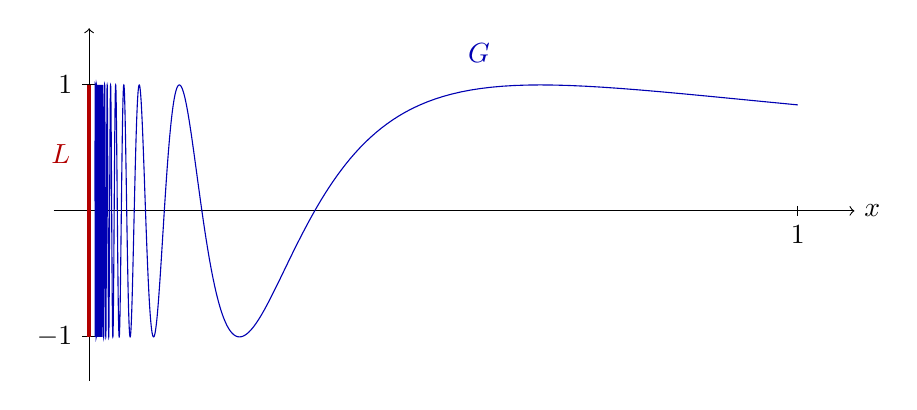
\begin{tikzpicture}[x=9cm, y=1.6cm]
    \draw[->] (-0.05,0) -- (1.08,0) node[right] {$x$};
    \draw[->] (0,-1.35) -- (0,1.45);
    \draw (1,0.04) -- (1,-0.04) node[below] {$1$};
    \draw (0.01,1) -- (-0.01,1) node[left] {$1$};
    \draw (0.01,-1) -- (-0.01,-1) node[left] {$-1$};
\draw[thin, blue!70!black] plot[domain=1:120, samples=2500, variable=\u] ({1/\u}, {sin(\u r)});
    \draw[very thick, red!70!black] (0,-1) -- (0,1);
    \node[blue!70!black] at (0.55,1.25) {$G$};
    \node[red!70!black] at (-0.04,0.45) {$L$};
  \end{tikzpicture}
  \end{center}
  \end{ergaenzung}
\end{example}


\begin{proof}[Beweis von Proposition~\ref{Zusammenhang}]
  \glqq$\fy$\grqq{} gilt stets. Ist $M$ ein zusammenhängender topologischer Raum und $\emptyset \neq C \subset M$ offen und abgeschlossen, so ist $C = M$.

  \glqq$\yf$\grqq: Sei $M$ eine zusammenhängende topologische $m$-dimensionale Mannigfaltigkeit. Zu zeigen ist, dass für alle $x, y \in M$ eine stetige Kurve $\gamma \in C^0([0, 1], M)$ mit $\gamma(0) = x$ und $\gamma(1) = y$ existiert. Anders gesagt reicht es zu zeigen, dass für alle $x \in M$
  \[ C_x \coloneqq \{ y \in M \mid \exists\, \gamma \in C^0([0, 1], M) \text{ mit } \gamma(0) = x,\ \gamma(1) = y \} \overset{!}{=} M. \]
\begin{ergaenzung}
  Wegen $x \in C_x$ (konstanter Weg) ist $C_x \neq \emptyset$.
  \end{ergaenzung}

  \textit{Behauptung 1: $C_x$ ist offen.} Sei $y \in C_x$ und $(U, \varphi)$ eine Karte nahe $y$. Da $\varphi(U) \subset \R^m$ offen ist, existiert ein Radius $\rho > 0$, sodass $B_\rho(\varphi(y)) \subset \varphi(U)$. Für jedes $z \in B_\rho(\varphi(y))$ ist $t \mapsto (1 - t)\varphi(y) + tz$ ein Weg in $C^0([0, 1], B_\rho(\varphi(y)))$, denn $B_\rho(\varphi(y)) \subset \R^m$ ist wegzusammenhängend. Definiere nun $\tilde{\gamma}\colon [0, 1] \to M$ durch
  \[ \tilde{\gamma}(t) \coloneqq \varphi^{-1}\bigl((1 - t)\varphi(y) + tz\bigr). \]
  Dann ist $\tilde{\gamma}$ stetig, weil $\varphi$ ein Homöomorphismus ist, und $\tilde{\gamma}$ verbindet $y$ mit $\varphi^{-1}(z) \in \varphi^{-1}(B_\rho(\varphi(y)))$. Wir haben also für jedes $y \in C_x$ eine offene Umgebung $\varphi^{-1}(B_\rho(\varphi(y)))$ gefunden, die wegzusammenhängend ist.
\begin{ergaenzung}
  Hängt man einen Weg von $x$ nach $y$ und $\tilde{\gamma}$ hintereinander, so erhält man einen Weg von $x$ nach $\varphi^{-1}(z)$. Also liegt die ganze Umgebung $\varphi^{-1}(B_\rho(\varphi(y)))$ in $C_x$.
  \end{ergaenzung}
  Also ist $C_x$ offen.


  \textit{Behauptung 2: $C_x$ ist abgeschlossen.} Sei $y \in M \setminus C_x$. Dann ist $C_y$ nach Behauptung~1 offen und eine Umgebung von $y$. Es reicht zu zeigen, dass $C_y \subset M \setminus C_x$, d.\,h. $C_y \cap C_x = \emptyset$. Andernfalls gäbe es ein $z \in C_x \cap C_y$, und man könnte $x$ über $z$ mit $y$ verbinden. Dann wäre $y \in C_x$, ein Widerspruch. Wegen $C_y \subset M \setminus C_x$ ist
  \[ M \setminus C_x = \bigcup_{y \in M \setminus C_x} C_y \]
  offen, also ist $C_x = M \setminus (M \setminus C_x)$ abgeschlossen.


  Da $M$ zusammenhängend ist, folgt $C_x = M$. Also ist $M$ wegzusammenhängend.
\end{proof}

\subsection{Beispiele differenzierbarer Strukturen}


\begin{example}
  $\{(\R, \id)\}$ ist ein $C^\infty$-Atlas auf $\R$. Ein weiterer $C^\infty$-Atlas ist $\{(\R, x \mapsto x^3)\}$. Allgemein bekommt man mit $\{(\R, \Phi)\}$ für jeden Homöomorphismus $\Phi\colon \R \to \R$ einen $C^\infty$-Atlas, denn die einzige Kartenwechselabbildung ist $\Phi \circ \Phi^{-1} = \id$, also $C^\infty$.

  Die zugehörigen differenzierbaren Strukturen sind aber im Allgemeinen verschieden. Zum Beispiel ist
  \[ \{(\R, \id), (\R, x \mapsto x^3)\} \]
  kein $C^1$-Atlas, weil für $\varphi = \id$ und $\psi(x) = x^3$ gilt: $(\varphi \circ \psi^{-1})(x) = x^{1/3} \notin C^1$.
\end{example}


\paragraph{Der projektive Raum $\R P^n$.}
Auf $\R^{n+1} \setminus \{0\}$ definiert man die Äquivalenzrelation
\[ x \sim y \iff \operatorname{span}\{x\} = \operatorname{span}\{y\}. \]
Damit ist $\R P^n \coloneqq (\R^{n+1} \setminus \{0\}) / {\sim}$ und $[x] = \operatorname{span}\{x\} \setminus \{0\}$ für $[x] \in \R P^n$.

\begin{proposition}[Projektiver Raum]\Theorem
  $\R P^n$ ist eine topologische Mannigfaltigkeit.
\end{proposition}

Die Topologie auf $\R P^n$ ist
\[ \{ \pi(U) : U \subset \R^{n+1} \setminus \{0\} \text{ offen} \}, \]
wobei $\pi\colon \R^{n+1} \setminus \{0\} \to \R P^n$, $x \mapsto [x]$, die kanonische Projektion ist.

\begin{lemma}[Hausdorff-Eigenschaft]\Theorem
  Die Topologie auf $\R P^n$ ist hausdorffsch.
\end{lemma}

\begin{proof}
  Seien $[x] \neq [y]$. Dann existiert ein $r > 0$, sodass $\operatorname{span} B_r(x) \cap \operatorname{span} B_r(y) = \{0\}$. Also ist $\pi(B_r(x)) \cap \pi(B_r(y)) = \emptyset$, d.\,h. $\pi(B_r(x))$ und $\pi(B_r(y))$ sind disjunkte Umgebungen von $[x]$ bzw. $[y]$.
\end{proof}


Nun geben wir noch einen Atlas an.

\begin{example}[Atlas für $\R P^1$]
  Setze
  \begin{align*}
    U_1 &\coloneqq \pi\bigl(\R^2 \setminus x_1\text{-Achse}\bigr), & \varphi_1\colon U_1 &\to \R, & \varphi_1([x]) &\coloneqq \frac{x_1}{x_2}, \\
    U_2 &\coloneqq \pi\bigl(\R^2 \setminus x_2\text{-Achse}\bigr), & \varphi_2\colon U_2 &\to \R, & \varphi_2([x]) &\coloneqq \frac{x_2}{x_1}.
  \end{align*}
  Dann ist $\{(U_1, \varphi_1), (U_2, \varphi_2)\}$ ein Atlas. Wegen $U_1 \cap U_2 = \pi(\R^2 \setminus \text{Achsen})$ ist $\varphi_1(U_1 \cap U_2) = \R \setminus \{0\}$, und die Übergangsabbildung
  \[ \varphi_2 \circ \varphi_1^{-1}\colon \varphi_1(U_1 \cap U_2) \to \R \setminus \{0\} \]
  ist $C^\infty$, denn $(\varphi_2 \circ \varphi_1^{-1})(t) = \frac{1}{t}$. Also ist dies ein $C^\infty$-Atlas.
\end{example}


\subsection{Differenzierbare Abbildungen}

\begin{definition}[Differenzierbare Abbildung]\Theorem
  Seien $M^m$ und $N^n$ beide $C^k$-Mannigfaltigkeiten. Eine Abbildung $f\colon M \to N$ heißt \emph{$C^k$}, wenn $f$ stetig ist und für alle Karten $(U, \varphi)$ eines Atlas auf $M$ und $(V, \psi)$ eines Atlas auf $N$
  \[ \psi \circ f \circ \varphi^{-1}\colon \varphi\bigl(U \cap f^{-1}(V)\bigr) \to \R^n \]
  eine $C^k$-Abbildung im üblichen Sinne ist.
\end{definition}

\begin{note}
  \begin{itemize}
    \item Damit sind auch $C^k$-Abbildungen auf $C^k$-Mannigfaltigkeiten erklärt.
    \item Ist $f$ eine $C^k$-Abbildung bezüglich eines Paares von Atlanten (auf $M$ und $N$), so auch bezüglich jedes anderen Paares jeweils äquivalenter Atlanten (Übungsaufgabe).
  \end{itemize}
\end{note}


\begin{definition}[Diffeomorphie]\Theorem
  Eine Abbildung $f\colon M \to N$ heißt \emph{$C^k$-Diffeomorphismus}, wenn $f$ ein Homöomorphismus ist und $f$ und $f^{-1}$ von der Klasse $C^k$ sind. Existiert ein $C^k$-Diffeomorphismus zwischen $M$ und $N$, so heißen $M$ und $N$ \emph{$C^k$-diffeomorph} zueinander.
\end{definition}


\begin{example}
  Sei $M = \R$ mit dem $C^\infty$-Atlas $\{(\R, \id)\}$ und $N = \R$ mit dem $C^\infty$-Atlas $\{(\R, \psi)\}$, $\psi(x) = x^{1/3}$. Das sind zwei verschiedene $C^\infty$-Mannigfaltigkeiten (siehe oben), aber sie sind diffeomorph: Für $f\colon M \to N$, $f(x) = x^3$, ist
  \[ \psi \circ f \circ \varphi^{-1} = \id, \]
  also $f \in C^\infty(M, N)$, und
  \[ \varphi \circ f^{-1} \circ \psi^{-1} = \id, \]
  also $f^{-1} \in C^\infty(N, M)$. Dabei ist $\varphi = \id$.
\end{example}


\begin{note}
  Ist $M$ eine Mannigfaltigkeit und $\varphi\colon M \to \varphi(M) \subset \R^m$ eine Karte, so ist $\varphi^{-1}\colon \varphi(M) \to M$ ein $C^k$-Diffeomorphismus von $(\varphi(M), \id)$ nach $M$ (Übungsaufgabe).
\end{note}


\begin{definition}[Immersion und Submersion]\Theorem
  Sei $f \in C^k(M, N)$. Dann heißt $f$ \emph{Immersion}, wenn $D(\psi \circ f \circ \varphi^{-1})(x)\colon \R^m \to \R^n$ für alle $x$ injektiv ist, und \emph{Submersion}, wenn diese Ableitung für alle $x$ surjektiv ist.
\end{definition}

\begin{note}
  Für eine Immersion muss $m \le n$ sein, für eine Submersion $m \ge n$. Die Definition ist wieder unabhängig von der Wahl der Atlanten innerhalb der differenzierbaren Struktur.
\end{note}

\section{Der Tangentialraum}

Für eine Untermannigfaltigkeit $M \subset \R^p$ ist der Tangentialraum im Punkt $x \in M$ definiert als
\[ T_x M \coloneqq \bigl\{ \gamma'(0) : \gamma \in C^1((-\delta, \delta), M),\ \gamma(0) = x \bigr\}. \]


\subsection{Tangentialraum von Untermannigfaltigkeiten}

\begin{note}
  Ist $M$ nahe $x_0 \in M$ als Niveaumenge einer Submersion $F\colon B_r(x_0) \to \R^{p-m}$ gegeben, so ist
  \[ T_{x_0} M = \ker DF(x_0). \]
\end{note}


\begin{example}
  Für $S^n \subset \R^{n+1}$ ist $S^n = F^{-1}(\{0\})$ mit $F(x) = \lvert x \rvert^2 - 1$. Wegen $\nabla F(x) = 2x$ ist $\ker DF(x) = \{x\}^\perp$, also $T_x S^n = \{x\}^\perp$.
\end{example}


\subsection{Tangentialraum von Mannigfaltigkeiten}

Sei nun $M^m$ eine $C^1$-Mannigfaltigkeit. Für $x_0 \in M$ definiere
\[ \mathcal{P}_{x_0}(M) \coloneqq \bigl\{ \gamma \in C^1((-\delta, \delta), M) : \delta > 0 \text{ und } \gamma(0) = x_0 \bigr\}. \]
Auf $\mathcal{P}_{x_0}(M)$ führt man die Äquivalenzrelation
\[ \gamma_1 \sim \gamma_2 \iff \text{es existiert eine Karte } (U, \varphi) \text{ nahe } x_0 \text{ mit } (\varphi \circ \gamma_1)'(0) = (\varphi \circ \gamma_2)'(0) \]
ein.


\begin{note}
  Es gilt $\gamma_1 \sim \gamma_2$ genau dann, wenn \textit{für alle} Karten nahe $x_0$ gilt: $(\varphi \circ \gamma_1)'(0) = (\varphi \circ \gamma_2)'(0)$.
\end{note}


\begin{proof}
  Übungsaufgabe.
\end{proof}

\begin{definition}[Tangentialraum]\Theorem
  Der \emph{Tangentialraum} an $M$ in $x_0$ ist
  \[ T_{x_0} M \coloneqq \mathcal{P}_{x_0}(M) / {\sim}. \]
\end{definition}


\section{Vektorfelder und Flüsse}

\subsection{Vektorfelder im \texorpdfstring{$\R^n$}{Rn}}

\begin{definition}[Vektorfeld]\Theorem
  Sei $U \subset \R^n$ offen. Eine Abbildung $X\colon U \to \R^n$ heißt \emph{Vektorfeld} auf $U$. Ist $X$ zudem $C^k$, so heißt $X$ ein \emph{$C^k$-Vektorfeld}.
\end{definition}


\begin{definition}[Integralkurve]\Theorem
  Sei $X$ ein $C^1$-Vektorfeld auf der offenen Menge $U \subset \R^n$. Eine $C^1$-Kurve $\gamma\colon I \to U$ auf einem offenen Intervall $I \subset \R$, die für alle $t \in I$ die Gleichung
  \[ \dot{\gamma}(t) = X\bigl(\gamma(t)\bigr) \]
  löst, heißt \emph{Integralkurve} des Vektorfeldes $X$.
\end{definition}


\begin{definition}[Fluss]\Theorem
  Sei $X$ ein $C^1$-Vektorfeld auf der offenen Menge $U \subset \R^n$ und $I \subset \R$ ein Intervall mit $0 \in I$. Eine Abbildung
  \[ \Gamma\colon I \times U \to U, \]
  die für alle $(t, x) \in I \times U$ den Gleichungen
  \begin{align*}
    \frac{\partial \Gamma}{\partial t}(t, x) &= X\bigl(\Gamma(t, x)\bigr), \\
    \Gamma(0, x) &= x
  \end{align*}
  genügt, heißt \emph{(lokaler) Fluss} von $X$.
\end{definition}


\begin{theorem}[lokale Existenz eines Flusses]\Theorem
  Sei $k \ge 1$, $X$ ein $C^k$-Vektorfeld auf der offenen Menge $U \subset \R^n$ und $a \in U$. Dann existieren eine offene Umgebung $\tilde{U} \subset U$ von $a$, ein $T > 0$ und eine $C^k$-Abbildung
  \[ \Gamma\colon [-T, T] \times \tilde{U} \to U, \]
  sodass für alle $(t, x) \in [-T, T] \times \tilde{U}$ gilt:
  \[ \frac{\partial \Gamma}{\partial t}(t, x) = X\bigl(\Gamma(t, x)\bigr), \qquad \Gamma(0, x) = x. \]
\end{theorem}




\PropertyNotice
\end{document}
